\documentclass[a4paper]{article}

%%%%%%%%%%%%%%%%%%%%%%%%%%%%%%%%%%%%%%%%%%%%%%
\usepackage[T1]{fontenc}
\usepackage{geometry}
\geometry{a4paper,left=1.5cm,right=1cm,top=1cm,bottom=1cm}

\usepackage{graphicx}
\usepackage[absolute,overlay]{textpos}
\usepackage{eso-pic}               % image de fond
\usepackage{fontawesome5}
\usepackage[hidelinks]{hyperref}
\usepackage{tikz}
\usepackage{xcolor}
\usepackage{enumitem}
\setlist{nosep,leftmargin=6mm}
\usepackage{times}                % même police que votre exemple
\usepackage{array} 
\usepackage{tabularx}
\usepackage{ragged2e}
\let\origcolorbox\colorbox    % sauvegarde
\renewcommand{\colorbox}[2]{#2}% neutralise le fond
%%%%%%%%%%%%%%%%%%%%%%%%%%%%%%%%%%%%%%%%%%%%%%
%\definecolor{texcolor}{HTML}{e2e8f0}
\providecolor{sidetext}{rgb}{1,1,1}
\definecolor{maincolor}{HTML}{ffffff}

%%%%%%%%%%%%%%%%%%%%%%%%%%%%%%%%%%%%%%%%%
% — Ne changez pas le nom : « background.jpg » doit être présent
\AddToShipoutPictureBG*{%
  
\includegraphics[width=\paperwidth,height=\paperheight]{background.jpg}%
}

%%%%%%%%%%%%%%%%%%%%%%%%%%%%%%%%%%%%%%%%%
\newcommand{\fullrule}{\hspace{-1.5cm}\rule{\paperwidth}{0.4pt}}
\newcommand{\cvsection}[1]{%
  \vspace{6pt}\textbf{\Large #1}\par\vspace{2pt}}
\newcommand{\cicon}[1]{%
  \tikz[baseline]{\draw[fill=white] (0,0.1) circle[radius=0.1cm];}~#1}

\setlength{\parindent}{0pt}
%\color{texcolor}
%%%%%%%%%%%%%%%%%%%%%%%%%%%%%%%%%%%%%%%%%%%%%%%%%%%%%%%%%%%%%%
\begin{document}
\color{white}
% ---------- Photo ------------------------------------------------
\begin{textblock*}{4cm}(0.2cm,0.3cm)
  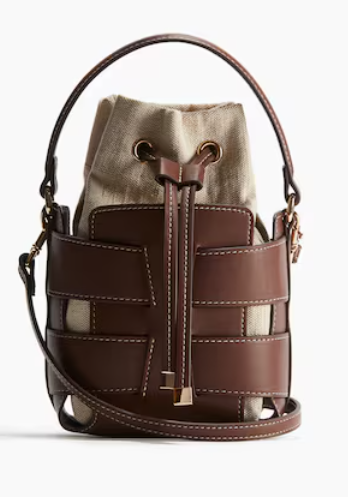
\includegraphics[width=2.5cm,clip,keepaspectratio]{25f5a781e1464e2b9c52ec9a38fa8e82.png}
\end{textblock*}

% ---------- En-tête ---------------------------------------------
\begin{center}
  {\fontsize{44pt}{24pt}\selectfont\bfseries Judikael Mourouvin}

  \bigskip
  {\Large Alternant Marketing Digital \& Informatique}

  \bigskip\bigskip
  \faMapMarker~Route de Cocoyer\ 97190 Gosier
  \quad\faEnvelope~\href{mailto:jkmou971@gmail.com}{jkmou971@gmail.com}

  \bigskip
  % Badge LinkedIn (retirez-le si inutile)
  \faPhone~ +590 0690 91 14 48
  \quad \faLinkedin\ \href{}{}
 

  \vspace{-0.3cm}
  \fullrule
\end{center}

% ---------- Profil ----------------------------------------------
\cvsection{Profil}

Passionné par l’informatique et le marketing digital, j’ai développé de solides compétences en configuration de postes, maintenance et diagnostic d’incidents. Mon année d’alternance à la DSI de la Mairie du Gosier m’a permis de gérer des projets numériques et d’accompagner les utilisateurs au quotidien. Je souhaite désormais m’investir à temps plein pour apporter mon savoir-faire technique et ma vision marketing à de nouveaux défis, avec rigueur et efficacité.

\medskip\fullrule

% ---------- Expérience ------------------------------------------
\cvsection{Expérience}
\hspace*{1.3cm}%

\colorbox{maincolor}{%
  \begin{minipage}{\linewidth}
    \textbf{Alternant en Marketing Digital} \\ Mairie du Gosier – DSI \\ 2023-2024
    \begin{itemize}
      \item Géré des projets numériques municipaux jusqu’à leur mise en production. \item Analysé les besoins des usagers et déployé des solutions adaptées, améliorant la satisfaction. \item Assuré support et formation des utilisateurs, renforçant l’adoption des outils digitaux.
    \end{itemize}
  \end{minipage}}

\vspace{3mm}


\colorbox{maincolor}{%
  \begin{minipage}{\linewidth}
    \textbf{Animateur de la zone informatique} \\ Pôle Emploi, Gosier \\ 2022-2023
    \begin{itemize}
      \item Fournit une assistance technique quotidienne, réduisant les incidents utilisateurs. \item Configuré et entretenu les postes de travail pour garantir une disponibilité optimale. \item Diagnostiqué et résolu les pannes, assurant la continuité de service.
    \end{itemize}
  \end{minipage}}

\vspace{3mm}


\colorbox{maincolor}{%
  \begin{minipage}{\linewidth}
    \textbf{Stagiaire Informaticien} \\ Numerika, Baie-Mahault \\ 2020-2021
    \begin{itemize}
      \item Installé et maintenu les équipements informatiques, assurant leur bon fonctionnement. \item Offert un support utilisateur de premier niveau pour accélérer la résolution des requêtes. \item Participé à la configuration réseau, contribuant à la stabilité de l’infrastructure.
    \end{itemize}
  \end{minipage}}

\medskip\fullrule

% ---------- Éducation -------------------------------------------
\cvsection{Éducation}
\hspace*{1.3cm}%

    \begin{tabularx}{\linewidth}{@{}c >{\RaggedRight\arraybackslash}X@{}}
    \textcolor{sidetext}{\faGraduationCap} &
    \textbf{Bachelor Marketing Digital} \\
    & CFA IUTS \\
    & \textit{2023-2024} \\
    \end{tabularx}
    \begin{itemize}[leftmargin=*]
  \item Étude des stratégies de communication en ligne et réseaux sociaux.
  \item Apprentissage des outils d’analyse de trafic et de performance.
  \item Projet pratique de conception de campagnes digitales.
\end{itemize}
\vspace{3mm}

    \begin{tabularx}{\linewidth}{@{}c >{\RaggedRight\arraybackslash}X@{}}
    \textcolor{sidetext}{\faGraduationCap} &
    \textbf{BTS Système Numérique option Informatique et Réseaux} \\
    & Lycée de Chevalier Saint Georges, Abymes \\
    & \textit{2019-2021} \\
    \end{tabularx}
    \begin{itemize}[leftmargin=*]
  \item Conception et administration de réseaux informatiques.
  \item Maintenance matérielle et logicielle de systèmes numériques.
  \item Développement de solutions embarquées et connectées.
\end{itemize}

\medskip\fullrule

% ---------- Compétences -----------------------------------------
\cvsection{Compétences}

\hspace*{2cm}%
\begin{tabular}{@{}p{0.25\linewidth}p{0.18\linewidth}p{0.18\linewidth}p{0.18\linewidth}}\cicon Administration & \cicon Réseaux & \cicon Support & \cicon Maintenance \\
\cicon Diagnostic & \cicon Configuration & \cicon Assistance & \cicon Marketing \\
\cicon Digital & \cicon Gestion & ~ & ~ \\\end{tabular}   % grille 3 lignes × 4 colonnes

\end{document}
